%!TeX root=../tese.tex
%("dica" para o editor de texto: este arquivo é parte de um documento maior)
% para saber mais: https://tex.stackexchange.com/q/78101/183146

%% ------------------------------------------------------------------------- %%
\chapter{Apresentação dos Resultados}
\label{cap:apresentacao}

Para determinar a efetividade do algoritmo genético, foram utilizados métodos estatísticos para comparar o desempenho do mesmo contra outros mecanismos de geração de oponentes. Para aproveitar melhor as características determinísticas do jogo \textit{Tower Defense}, os experimentos se concentraram no mesmo, pois a natureza mais aleatória do \textit{Space Shooter} produziu resultados mais difíceis de analisar e, infelizmente, não havia mais tempo disponível para ajustar os cenários e função \textit{fitness} ou taxa de mutação até encontrar resultados mais conclusivos.

%% ------------------------------------------------------------------------- %%
\section{Organização dos dados}
\label{sec:a-organizacao}

A análise dos dados partiu das estatísticas descritivas de cada onda para todos os experimentos executados, conforme ilustrado pela Tabela \ref{tab:colunas}; isto é, foram obtidos 30 amostras de dano para cada i-ésima onda.

\begin{table}
\caption{Forma de coleta dos dados de cada onda.}
\begin{tabular}{l|l|l|l|l|l|l}
\cline{2-6}
               & onda 1 & onda 2 & ... & onda n - 1 & onda n \\ \cline{2-6}
experimento 1  &        &        &     &            &         \\
experimento 2  &  dano  &  dano  &     &  dano      &  dano   \\
...            &  da    &  da    & ... &  da        &  da     \\
experimento 29 &  onda  &  onda  &     &  onda      &  onda   \\
experimento 30 &        &        &     &            &         \\ \cline{2-6}
\end{tabular}
\label{tab:colunas}
\end{table}

%% ------------------------------------------------------------------------- %%
\section{Dados das Ondas}
\label{sec:a-ondas}

As seções seguintes irão dispor os dados considerados relevantes para análise de desempenho do algoritmo, obtidos através da análise exploratória de dados pelos \textit{Jupyter Notebook}\footnote{Repositório disponível em \url{https://github.com/raktanaka/tcc-results} - 24/12/2021} desenvolvidos. Dados de ondas sempre com o mesmo tipo de inimigos - chamadas de ondas repetidas - podem mostrar uma possível solução maximal ou próxima dela, para a qual o algoritmo poderia convergir. Já os dados de ondas com inimigos escolhidos ao acaso - chamadas de ondas aleatórias - indicam um possível valor de dano mínimo, que seria atingido com um método que também não precisa de conhecimento das mecânicas de jogo e de informações sobre os inimigos disponibilizadas.

Para visualização do funcionamento dos algoritmos, foram geradas imagens com as modas\footnote{Valores mais frequentes em um conjunto de dados} das ondas geradas a partir dos arquivos de texto com os dados. Um \textit{notebook} faz os cálculo necessários e utiliza a biblioteca \textit{Matplotlib} para produzir a imagem com os \textit{sprites} e caminho ou localização do inimigo. As figuras fornecem os inimigos mais comuns em cada onda, mostrando para qual solução o algoritmo tende a convergir. Estas estão disponíveis nos apêndices \ref{sec:apend-moda-td-v1}, \ref{sec:apend-moda-td-v2}, \ref{sec:apend-moda-td-v3}, \ref{sec:apend-moda-ss-v1}, \ref{sec:apend-moda-ss-v3}.

%% ------------------------------------------------------------------------- %%
\subsection{Tower Defense - Ondas Repetidas}
\label{sec:uni-td}

Seguem os dados obtidos nos experimentos feito no jogo, para facilidade de leitura, uma cópia da tabela \ref{tab:tank-dmg} da seção \ref{sec:mj-td} está abaixo.

\begin{table}
\caption{Dano de cada tanque no Tower Defense}
\begin{tabular}{c|cc}
            & velocidade & dano   \\ \hline
tank blue   & 55    & 55         \\
tank green  & 70    & 45         \\
tank red    & 80    & 15          \\
tank orange & 120   & 5           \\
tank purple & 90    & 15          \\
tank yellow & 150   & 5           
\end{tabular}
\label{tab:tank-dmg3}
\end{table}

Através da Tabela \ref{tab:tank-dmg3} é possível calcular o dano máximo possível como produto dos 12 inimigos que podem ser gerados por \textit{wave} e do maior dano disponível:
\[12 * 55 = 660\]
Numa onda composta inteiramente por tanques verdes (\textit{EnemyGreen}), sem nenhuma eliminação. As Tabelas \ref{tab:green}, \ref{tab:red}, \ref{tab:greenred} e \ref{tab:redgreen} a seguir mostram os dados de dano médio para cada onda e cada tipo de inimigo, obtidos através das simulações do jogo.

\begin{table}
\caption{Desempenho das \textbf{ondas repetidas} contra Torres \textbf{exclusivamente Verdes}}
\begin{tabular}{l|l|ll}
Torres & Inimigos & Dano Médio & Desvio Padrão \\ \hline
Verdes & EnemyGreen    & 450.00     & 0.0           \\
Verdes & OneEach       & 122.35     & 4.52          \\
Verdes & EnemyPurple   & 90.06      & 0.91          \\
Verdes & EnemyRed      & 89.90      & 1.22          \\
Verdes & EnemyBlue     & 60.68      & 16.77         \\
Verdes & EnemyYellow   & 40.07      & 0.57          \\
Verdes & EnemyOrange   & 39.93      & 0.57         
\end{tabular}
\label{tab:green}
\end{table}

Conforme os dados gerados para torres exclusivamente verdes, nota-se que tanques verdes possuem maior facilidade em causar dano ao jogador, uma vez que possuem a mecânica de \textbf{Resistência} contra torres da mesma cor que eles. Portanto, no algoritmo genético, espera-se que esses sejam os indivíduos mais numerosos da população final.

\begin{table}
\caption{Desempenho das \textbf{ondas repetidas} contra Torres \textbf{exclusivamente Vermelhas}}
\begin{tabular}{l|l|ll}
Torres    & Inimigos & Dano Médio & Desvio Padrão \\ \hline
Vermelhas & EnemyGreen    & 360.00     & 0.0           \\
Vermelhas & EnemyBlue     & 355.85     & 28.58         \\
Vermelhas & EnemyRed      & 180.00     & 0.0           \\
Vermelhas & OneEach       & 167.82     & 2.48          \\
Vermelhas & EnemyPurple   & 127.60     & 8.54          \\
Vermelhas & EnemyYellow   & 50.58      & 1.61          \\
Vermelhas & EnemyOrange   & 50.00      & 0.0          
\end{tabular}
\label{tab:red}
\end{table}

Os dados gerados para torres exclusivamente vermelhas apresenta que, em média,  tanques Verdes e Azuis são os melhores causadores de dano por onda, mesmo com a resistência dos tanques vermelhos sobre as torres vermelhas. Essa disparidade ocorre pela quantidade de dano que os tanques causam ao chegar no inimigo, conforme Tabela \ref{tab:tank-dmg3}, o tanque vermelho causa 15 de dano, ou seja, os 12 ($\frac{180}{15}$) tanques sobrevivem ao final de todas as ondas. Contudo, os inimigos verdes e azuis causam mais dano, mesmo que cheguem menos tanques ao final do trajeto, 8 ($\frac{360}{45}$) para tanques verdes e entre 6-7 ($\frac{355}{55}$) nos azuis. 

\begin{table}
\caption{Desempenho das \textbf{ondas repetidas} contra \textbf{1 Torre Verde e 1 Vermelha} (Nessa ordem)}
\begin{tabular}{l|l|ll}
Torres           & Inimigos & Dano Médio & Desvio Padrão \\ \hline
Verde + Vermelha & EnemyGreen    & 420.20     & 13.91         \\
Verde + Vermelha & EnemyBlue     & 220.18     & 3.18          \\
Verde + Vermelha & EnemyRed      & 148.50     & 4.50          \\
Verde + Vermelha & OneEach       & 148.45     & 4.57          \\
Verde + Vermelha & EnemyPurple   & 120.00     & 0.0           \\
Verde + Vermelha & EnemyYellow   & 50.00      & 0.0           \\
Verde + Vermelha & EnemyOrange   & 44.50      & 1.50          
\end{tabular}
\label{tab:greenred}
\end{table}

\pagebreak

Conforme as informações da Tabela \ref{tab:greenred}, percebe-se que o inimigo Verde tem o melhor desempenho de dano por onda repetida, mesmo que sobrevivam menos indivíduos ao final em comparação ao inimigo Vermelho, uma vez que o dano de Verde é 3 vezes maior. Chegam ao final, aproximadamente 9 ($\frac{420}{45}$) Verdes e 10 Vermelhos ($\frac{148.5}{15}$). 

\begin{table}[H]
\caption{Desempenho das \textbf{ondas repetidas} contra \textbf{1 Torre Vermelha e 1 Verde}(Nessa ordem)}
\begin{tabular}{l|l|ll}
Torres            & Inimigos & Dano Médio & Desvio Padrão \\ \hline
Vermelha + Verde  & EnemyGreen      & 449.85     & 2.60          \\
Vermelha + Verde  & EnemyBlue       & 329.82     & 3.18          \\
Vermelha + Verde  & EnemyRed        & 149.90     & 1.73          \\
Vermelha + Verde  & OneEach         & 135.05     & 0.87          \\
Vermelha + Verde  & EnemyPurple     & 120.00     & 0.0           \\
Vermelha + Verde  & EnemyYellow     & 50.00      & 0.0           \\
Vermelha + Verde  & EnemyOrange     & 49.45      & 1.57          
\end{tabular}
\label{tab:redgreen}
\end{table}

Para a Tabela \ref{tab:redgreen}, nota-se um aumento de desempenho significativo do inimigo Azul e Verde, onde sobrevive um tanque a mais verde e quase 2 azuis em relação ao anterior. Contudo, mantém-se a dominância do dano médio por onda do inimigo Verde. Os desvios padrões baixos - o mais alto apresentado nas Torres Verdes contra \textit{EnemyBlue} é de aproximadamente 25\% do dano total, mas é uma exceção considerando todos os resultados - mostram a consistência do jogo.

Conforme os dados gerados, o inimigo Verde indica ter o melhor desempenho de dano nas ondas repetidas, contudo, mais para frente desse capítulo, será mostrado que eles não serão os mais selecionados, por conta da função \textit{fitness} escolhida, que prioriza sobrevivência ao invés de dano por \textit{wave}.

%% ------------------------------------------------------------------------- %%
\subsection{Tower Defense - Ondas Aleatórias}
\label{sec:rd-td}

Foram calculadas as médias de dano causadas por cada onda aleatória de distribuição uniforme (Tabela \ref{tab:td-rd-avg}) e o máximo de dano causado em qualquer onda (Tabela \ref{tab:td-rd-max}), considerando todos os experimentos. A Figura \ref{fig:td-rd-max} ilustra a onda que causou o maior dano.

\begin{table}
\begin{tabular}{l|ll}
Torres            & Dano Médio & Desvio Padrão \\ \hline
Verdes            & 81.42      & 55.00         \\
Vermelhas         & 125.35     & 56.98         \\
Verde + Vermelha  & 100.37     & 54.16         \\
Vermelha + Verde  & 102.37     & 56.62          
\end{tabular}
\caption{Média e Desvio Padrão do dano em ondas aleatórias no Tower Defense.}
\label{tab:td-rd-avg}
\end{table}

\pagebreak

\begin{table}
\centering
\begin{tabular}{p{1.7cm}|l|p{1.0cm}}
Torres                   & Onda                                                                                                                         & Dano \newline Total \\ \hline
Verdes                   & \begin{tabular}{@{}c@{}} {[}EnemyGreen, 1{]}; {[}EnemyGreen, 1{]}; {[}EnemyGreen, 0{]}; {[}EnemyRed, 1{]};     \\
                                                    {[}EnemyPurple, 0{]}; {[}EnemyGreen, 0{]}; {[}EnemyRed, 1{]}; {[}EnemyGreen, 0{]};    \\
                                                    {[}EnemyOrange, 0{]}; {[}EnemyGreen, 0{]}; {[}EnemyGreen, 0{]}; {[}EnemyRed, 0{]}     \end{tabular} & 290        \\ \hline
Vermelhas                & \begin{tabular}{@{}c@{}} {[}EnemyBlue, 0{]}; {[}EnemyRed, 0{]}; {[}EnemyBlue, 0{]}; {[}EnemyGreen, 0{]};       \\
                                                    {[}EnemyGreen, 1{]}; {[}EnemyRed, 1{]}; {[}EnemyBlue, 0{]}; {[}EnemyOrange, 1{]};     \\
                                                    {[}EnemyBlue, 0{]}; {[}EnemyYellow, 0{]}; {[}EnemyOrange, 0{]}; {[}EnemyYellow, 1{]}  \end{tabular} & 355        \\ \hline
Verde + \newline Vermelha & \begin{tabular}{@{}c@{}} {[}EnemyPurple, 0{]}; {[}EnemyBlue, 0{]}; {[}EnemyBlue, 0{]}; {[}EnemyBlue, 1{]};    \\
                                                     {[}EnemyRed, 0{]}; {[}EnemyGreen, 1{]}; {[}EnemyYellow, 0{]}; {[}EnemyRed, 1{]};     \\
                                                     {[}EnemyGreen, 1{]}; {[}EnemyGreen, 0{]}; {[}EnemyGreen, 0{]}; {[}EnemyYellow, 1{]}  \end{tabular} & 330        \\ \hline
Vermelha \newline + Verde & \begin{tabular}{@{}c@{}} {[}EnemyYellow, 0{]}; {[}EnemyBlue, 0{]}; {[}EnemyRed, 1{]}; {[}EnemyGreen, 0{]};    \\
                                                     {[}EnemyGreen, 1{]}; {[}EnemyRed, 1{]}; {[}EnemyGreen, 0{]}; {[}EnemyYellow, 0{]};   \\
                                                     {[}EnemyRed, 1{]}; {[}EnemyGreen, 0{]}; {[}EnemyGreen, 0{]}; {[}EnemyPurple, 1{]}    \end{tabular} & 315       
\end{tabular}
\caption{Ondas aleatórias com maior dano no Tower Defense.}
\label{tab:td-rd-max}
\end{table}

\begin{figure}
  \centering
  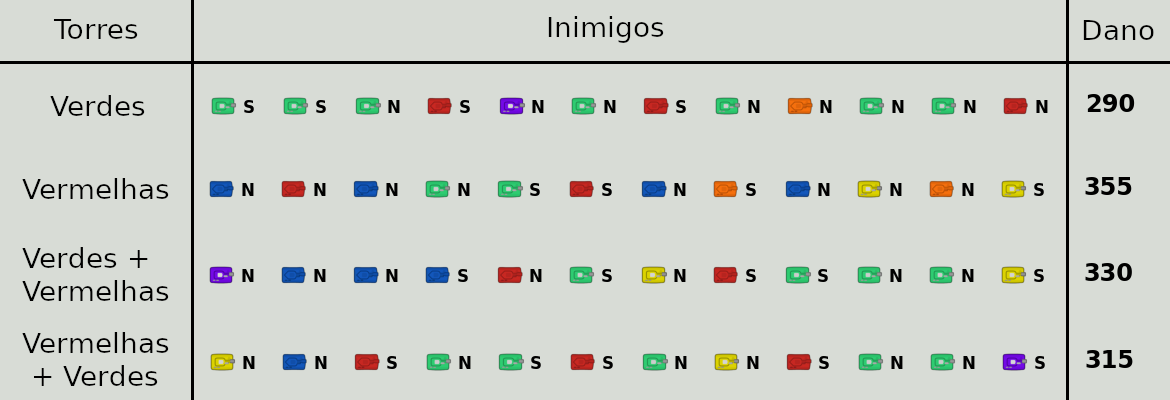
\includegraphics[width=1.0\textwidth]{td/tab-rd-max.png}
  \caption{Visualização das ondas aleatórias com maior dano no Tower Defense.}
  \label{fig:td-rd-max}
\end{figure}

%% ------------------------------------------------------------------------- %%
\subsection{Space Shooter - Ondas Repetidas}
\label{sec:uni-ss}


Foram executados experimentos análogos ao \textit{Tower Defense} no \textit{Space Shooter}, segue uma cópia da tabela \ref{tab:ss-ast-dmg} da seção \ref{sec:mj-ss} para facilitar leitura.

\begin{table}[H]
\caption{Velocidade, dano e vida de cada asteroide no Space Shooter}
\begin{tabular}{c|ccc}
         & Velocidade & Dano & Vida   \\ \hline
inimigos & 500        & 20     &   50     \\
inimigo1 & 350        & 45     &   30     \\
inimigo2 & 470        & 50     &   40     \\
inimigo3 & 320        & 60     &   40     \\
inimigo4 & 550        & 20     &   60     \\
inimigo5 & 700        & 10     &   120      
\end{tabular}
\label{tab:ss-ast-dmg-copia}
\end{table}

\pagebreak

Através da Tabela \ref{tab:ss-ast-dmg-copia}, é possível calcular o dano máximo possível como a onda de seis inimigos com o maior dano disponível:
\[6 * 60 = 360\]
Numa onda composta inteiramente pelo \textit{inimigo3}, sem nenhuma eliminação. As tabelas \ref{tab:ss-yellow-still}, \ref{tab:ss-yellow-move}, \ref{tab:ss-red-still} e \ref{tab:ss-red-move} a seguir mostram os dados de dano médio para cada onda e cada tipo de inimigo.

\begin{table}
\centering
\caption{\textbf{Ondas repetidas} contra IA de \textbf{Disparo Amarelo} e \textbf{Parado}} .
\begin{tabular}{l|l|ll}
Nave                     & Inimigo  & Dano Médio & Desvio Padrão \\ \hline
Disparo Amarelo - Parada & Inimigo3 & 314.93     & 42.46         \\
Disparo Amarelo - Parada & Inimigo2 & 299.78     & 3.33          \\
Disparo Amarelo - Parada & Inimigo1 & 181.50     & 41.67         \\
Disparo Amarelo - Parada & Inimigo4 & 120.00     & 0.0           \\
Disparo Amarelo - Parada & Inimigos & 120.00     & 0.0           \\
Disparo Amarelo - Parada & OneEach  & 82.75      & 27.47         \\
Disparo Amarelo - Parada & Inimigo5 & 60.00      & 0.0          
\end{tabular}
\label{tab:ss-yellow-still}
\end{table}

Na tabela, nota-se que os valores piores classificados são as ondas em que todos os asteroides chegaram no Jogador, mas possuem danos muito baixos ($\frac{\text{dano médio}}{\text{dano individual do asteróide}}$), enquanto os que possuem danos melhores perderam algum indivíduo da população no caminho, pois possuem valores menores que os danos totais possíveis (dano * 6, onde 6 é quantidade de inimigos) e seu desvio padrão é alto.

\begin{table}
\centering
\caption{\textbf{Ondas repetidas} contra IA de \textbf{Disparo Amarelo} e \textbf{Movendo}}.
\begin{tabular}{l|l|ll}
Nave                      & Inimigo  & Dano Médio & Desvio Padrão \\ \hline
Disparo Amarelo - Movendo & Inimigo3 & 213.20     & 52.43         \\
Disparo Amarelo - Movendo & Inimigo2 & 184.61     & 41.98         \\
Disparo Amarelo - Movendo & Inimigo1 & 130.10     & 48.15         \\
Disparo Amarelo - Movendo & OneEach  & 100.85     & 43.75         \\
Disparo Amarelo - Movendo & Inimigo4 & 80.69      & 15.70         \\
Disparo Amarelo - Movendo & Inimigos & 67.69      & 15.46         \\
Disparo Amarelo - Movendo & Inimigo5 & 39.23      & 7.71         
\end{tabular}
\label{tab:ss-yellow-move}
\end{table}

Para esses dados, nota-se que, com a Nave se movendo, a chance dos inimigos acertarem o Jogador decai bastante em todos os casos, contudo, os tipos de inimigos mais promissores ainda se mantém como Inimigo3, Inimigo2 e Inimigo1.

\pagebreak

\begin{table}
\centering
\begin{tabular}{l|l|ll}
Nave                      & Inimigo  & Dano Médio & Desvio Padrão \\ \hline
Disparo Vermelho - Parada & Inimigo3 & 241.60     & 56.01         \\
Disparo Vermelho - Parada & Inimigo2 & 240.94     & 56.09         \\
Disparo Vermelho - Parada & OneEach  & 125.99     & 38.03         \\
Disparo Vermelho - Parada & Inimigo4 & 106.00     & 21.81         \\
Disparo Vermelho - Parada & Inimigos & 102.44     & 20.04         \\
Disparo Vermelho - Parada & Inimigo5 & 62.57      & 17.74         \\
Disparo Vermelho - Parada & Inimigo1 & 27.60      & 29.54        
\end{tabular}
\caption{\textbf{Ondas repetidas} contra IA de \textbf{Disparo Vermelho} e \textbf{Parado} \label{tab:ss-red-still}}.
\end{table}

Para esses dados, percebe-se que o Disparo Vermelho tem uma vantagem muito maior contra \textbf{Inimigo1}, um dos candidatos para o indivíduo mais apto da população nos testes para o Disparo Amarelo, principalmente por matá-lo em um único disparo.

\begin{table}
\centering
\caption{\textbf{Ondas repetidas} contra IA de \textbf{Disparo Vermelho} e \textbf{Movendo}}.
\begin{tabular}{l|l|ll}
Nave                       & Inimigo  & Dano Médio & Desvio Padrão \\ \hline
Disparo Vermelho - Movendo & Inimigo3 & 169.87     & 63.54         \\
Disparo Vermelho - Movendo & Inimigo2 & 169.67     & 49.77         \\
Disparo Vermelho - Movendo & OneEach  & 96.99      & 39.72         \\
Disparo Vermelho - Movendo & Inimigo4 & 76.29      & 18.05         \\
Disparo Vermelho - Movendo & Inimigos & 65.89      & 18.23         \\
Disparo Vermelho - Movendo & Inimigo5 & 39.26      & 7.40          \\
Disparo Vermelho - Movendo & Inimigo1 & 24.60      & 28.60        
\end{tabular}
\label{tab:ss-red-move}
\end{table}

Novamente, a classificação dos indivíduos que parecem mais aptos não muda muito, somente decai o Dano Médio por onda já que a Nave agora está se \textbf{movendo}, dificultando que os asteroides a acertem.

Essas tabelas das ondas repetidas são importantes pois ajudam a inferir sobre os resultados que levaram aos indivíduos na população final após a execução do algoritmo genético. Também mostram, através dos desvios padrões altos - diversos testes mostram valores que chegam a ser maiores que o dano médio - bastante acima dos obtidos no \textit{Tower Defense} que a variabilidade de cada onda é alta, e irá interferir nos resultados.

%% ------------------------------------------------------------------------- %%
\subsection{Space Shooter - Ondas Aleatórias}
\label{sec:rd-ss}

Foram calculadas as médias de dano causado por cada onda aleatória (Tabela \ref{tab:ss-rd-avg}) e o máximo de dano causado em qualquer onda (Tabela \ref{tab:ss-rd-max}), considerando todos os experimentos. A Figura \ref{fig:ss-rd-max} ilustra a onda que causou o maior dano, um resultado importante para embasar que o Algoritmo Genético possui um desempenho melhor do que Ondas de Distribuição Uniforme Aleatórias.

\begin{table}
\begin{tabular}{l|ll}
Nave                        & Dano Médio & Desvio Padrão \\ \hline
Disparo Amarelo - Parada    & 181.26     & 46.18         \\
Disparo Amarelo - Movendo   & 124.95     & 47.32         \\
Disparo Vermelho - Parada   & 123.66     & 50.84         \\
Disparo Vermelho - Movendo  & 91.77      & 46.11          
\end{tabular}
\caption{Média e Desvio Padrão do dano em \textit{ondas aleatórias} no Space Shooter.}
\label{tab:ss-rd-avg}
\end{table}



\begin{table}
\centering
\begin{tabular}{p{1.9cm}|l|p{1.0cm}}
Nave                       & Onda                                                                                              & Dano Total \\ \hline
Disparo Amarelo - Parada   & \begin{tabular}{@{}c@{}} {[}inimigo1, (-100, 300){]}; {[}inimigo3, (-100, 100){]};  \\
                                                      {[}inimigo1, (-100, 300){]}; {[}inimigo1, (-100, 300){]};  \\
                                                      {[}inimigos, (90, -50){]}; {[}inimigo3, (-100, 100){]}     \end{tabular} & 275        \\ \hline
Disparo Amarelo - Movendo  & \begin{tabular}{@{}c@{}} {[}inimigo3, (-100, 100){]}; {[}inimigo1, (-100, 300){]};  \\
                                                      {[}inimigo3, (-100, 100){]}; {[}inimigo1, (-100, 300){]};  \\
                                                      {[}inimigo1, (-100, 300){]}; {[}inimigo3, (-100, 100){]}   \end{tabular} & 315        \\ \hline
Disparo Vermelho - Parada  & \begin{tabular}{@{}c@{}} {[}inimigo3, (-100, 100){]}; {[}inimigo3, (-100, 100){]};  \\
                                                      {[}inimigo5, (1350, 500){]}; {[}inimigo4, (200, -50){]};   \\
                                                      {[}inimigo3, (-100, 100){]}; {[}inimigo2, (1350, 100){]}   \end{tabular} & 260        \\ \hline
Disparo Vermelho - Movendo & \begin{tabular}{@{}c@{}} {[}inimigo3, (90, -50){]}; {[}inimigo1, (90, -50){]};      \\
                                                      {[}inimigo3, (90, -50){]}; {[}inimigo1, (90, -50){]};      \\
                                                      {[}inimigo5, (90, -50){]}; {[}inimigo1, (90, -50){]}       \end{tabular} & 350       
\end{tabular}
\caption{\textbf{Ondas aleatórias} com maior dano no Space Shooter.
\label{tab:ss-rd-max}}
\end{table}

\begin{figure}
  \centering
  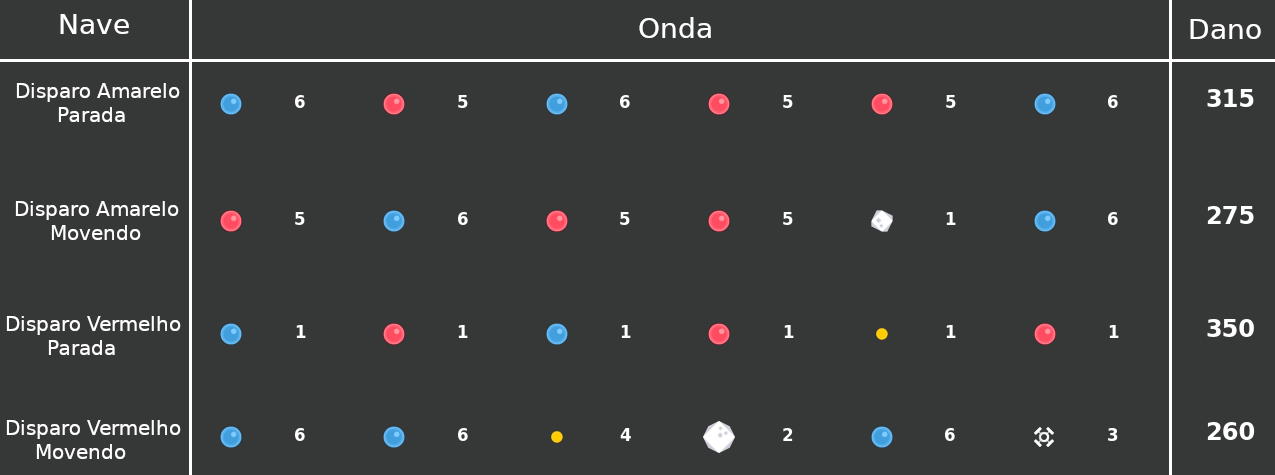
\includegraphics[width=1.0\textwidth]{ss/tab-ss-max.png}
  \caption{Visualização das ondas aleatórias com maior dano no Space Shooter.\label{fig:ss-rd-max}}
\end{figure}

\pagebreak

%% ------------------------------------------------------------------------- %%
\section{Fitness dos Jogos}
\label{sec:a-fitness}

\subsection{Fitness e Mutação}
\label{sec:a-fitness-mutacao-usados}

Foram testados três modelos de \textit{fitness} no algoritmo genético para o jogo \textit{Tower Defense}, buscando obter melhores resultados na geração de ondas; enquanto o jogo \textit{Space Shooter} foi testado somente com a primeira e a terceira versão. Foi adotada uma nomenclatura de versões para simplificar as referências no texto:

\begin{table}
\centering
\begin{tabular}{l|l|l}
                            & \textit{Fitness} (v1) & \textit{Fitness} (v2)  \\ \hline
Taxa de mutação (v1)             & TD e SS          & -                      \\
Taxa de mutação (v2)             &      -           & TD                     \\
Taxa de mutação (v3)             &      SS          & TD          

\end{tabular}
\caption{Relação dos fitness e taxa de mutação usados no TD e SS.}
\label{tab:fit-names}
\end{table}

%% ------------------------------------------------------------------------- %%
\subsection{Tower Defense - Fitness e Mutação}
\label{sec:td-fit}

O primeiro teste realizado utilizou uma função \textit{fitness} que considera se o alvo chegou ao final do trajeto e o quanto do trajeto foi percorrido, indivíduos que completaram o percurso serão muito mais recompensados e aqueles que morreram muito longe do alvo tendem a ser eliminados da população. A taxa de mutação decai conforme o tempo, começando em \textit {mutation\_prob} = 1.0 (100\%) e decrementando até 0. A taxa de mutação volta para 100\% a cada repetição do experimento (30 ondas). 

\begin{programruledcaption}{\textit{Fitness} do primeiro teste do \textit{TD} (v1).\label{prog:avaliacao_TD1}}
  \begin{lstlisting}[
    language={[brazilian]pseudocode},
    style=pseudocode,
    style=wider,
    functions={},
    specialidentifiers={},
  ]
        funcao fitness_v1 (x) // Dá uma pontuação para indivíduo \textbf{x}
            // reached\_goal(x) = booleana se chegou ou não ao final do trajeto
            se reached_goal(x)
                fit := 1
            senao
                fit := 0
            
            // offset(x) = quanto do percurso foi completado.
	        fit := (fit + offset(x)) / 2 // média aritmética dos valores de x
	        devolva fit // Um float com uma pontuação no intervalo [0,1].
        fim
  \end{lstlisting}
\end{programruledcaption}

\begin{programruledcaption}{Taxa de mutação do \textit{TD} para o primeiro teste (v1).\label{prog:mutacao_TD1}}
  \begin{lstlisting}[
    language={[brazilian]pseudocode},
    style=pseudocode,
    style=wider,
    functions={},
    specialidentifiers={},
  ]
        funcao mutation_v1 () 
            se mutation_prob >= 0
		        mutation_prob -= 0.05
		    ...
		    // continuação do processo de mutação.
        fim
  \end{lstlisting}
\end{programruledcaption}

Para o segundo teste, a função \textit{fitness} considera a quantidade do trajeto que foi percorrido (\textit{float} de 0 a 1) e a quantidade de vida ao final do trajeto (\textit{float} de 0 a 1), ou seja, inimigos que completarem o percurso serão mais recompensados conforme a quantidade de vida que chegaram ao final do trajeto. Note que indivíduos que morreram no caminho não serão bem recompensados com essa função. Por um erro, a taxa de mutação ficou em 1 a partir da segunda wave, contudo, alguns resultados interessantes foram obtidos também.

\begin{programruledcaption}{\textit{Fitness} do \textit{TD} (v2) (Avaliação, em português).\label{prog:avaliacao_TD2}}
  \begin{lstlisting}[
    language={[brazilian]pseudocode},
    style=pseudocode,
    style=wider,
    functions={},
    specialidentifiers={},
  ]
        funcao fitness_TD_v2 (x) // Dá uma pontuação para indivíduo \textbf{x}
            // offset(x) = quanto do trajeto foi percorrido, float de 0 a 1.
            // hp (x) = quanto de HP sobrou do inimigo, float de 0 a 1.
	        fit := (offset(x) + hp(x)) / 2 // média aritmética dos valores de x
	        devolva fit // Pontuação no intervalo [0,1].
        fim
  \end{lstlisting}
\end{programruledcaption}


\begin{programruledcaption}{Taxa de mutação do \textit{TD} para cada bateria de testes (2º par dos gráficos).\label{prog:mutacao_TD2}}
  \begin{lstlisting}[
    language={[brazilian]pseudocode},
    style=pseudocode,
    style=wider,
    functions={},
    specialidentifiers={},
  ]
        funcao mutation_v2 () 
            se geração = 1
		        mutation_prob := 1 / 12
		        
		    senão
		        mutation_prob := 1.0
		    ...
		    // continuação do processo de mutação.
        fim
  \end{lstlisting}
\end{programruledcaption}

Para o terceiro teste, a função \textit{fitness} considera a quantidade do trajeto que foi percorrido (float de 0 a 1) e a quantidade de vida ao final do trajeto (float de 0 a 1), idêntico ao anterior. Contudo, a taxa de mutação permanece em um valor fixo equivalente a $\frac{1}{12}$, conforme embasamento no estudo de \citet{haupt00:mutationprob}.

\begin{programruledcaption}{\textit{Fitness} do \textit{TD} (v3) (Avaliação, em português).\label{prog:avaliacao_TD3}}
  \begin{lstlisting}[
    language={[brazilian]pseudocode},
    style=pseudocode,
    style=wider,
    functions={},
    specialidentifiers={},
  ]
        funcao fitness_TD_v3 (x) // Dá uma pontuação para indivíduo \textbf{x}
            // offset (x) = quanto do trajeto foi percorrido, float de 0 a 1.
            // hp (x) = quanto de HP sobrou do inimigo, float de 0 a 1.
	        fit := ( offset (x) + hp (x)) / 2 // média aritmética dos valores de x
	        devolva fit // Pontuação no intervalo [0,1].
        fim
  \end{lstlisting}
\end{programruledcaption}

\begin{programruledcaption}{Taxa de mutação  v3 do \textit{TD} para cada bateria de testes (3º par dos gráficos).\label{prog:mutacao_TD3}}
  \begin{lstlisting}[
    language={[brazilian]pseudocode},
    style=pseudocode,
    style=wider,
    functions={},
    specialidentifiers={},
  ]
        funcao mutation_v3 () 
            mutation_prob := 1 / 12
		    ...
		    // continuação do processo de mutação.
        fim
  \end{lstlisting}
\end{programruledcaption}

%% ------------------------------------------------------------------------- %%
\subsection{Space Shooter - Fitness e Mutação}
\label{sec:ss-fit}

Conforme a Tabela \ref{tab:fit-names}, temos uma única função \textit{fitness} e as mesmas taxas de mutação 1 e 2 apresentadas na subseção anterior.

\begin{programruledcaption}{\textit{Fitness} de todos os testes do \textit{SS} (v1).\label{prog:avaliacao_SS1}}
  \begin{lstlisting}[
    language={[brazilian]pseudocode},
    style=pseudocode,
    style=wider,
    functions={},
    specialidentifiers={},
  ]
        funcao fitness_v1 (x) // Dá uma pontuação para indivíduo \textbf{x}
            // reached\_goal(x) = booleana se acertou o inimigo
            se reached_goal(x)
                fit := 5
            senao
                fit := 0
            
            // hp (x) = 5 * quanto de HP restou ao final da rodada.
	        fit := (fit + hp (x)) / 10 // média aritmética dos valores de x
	        devolva fit // Um float com uma pontuação no intervalo [0,1].
        fim
  \end{lstlisting}
\end{programruledcaption}%CONSERTADO, EU ACHO


%% ------------------------------------------------------------------------- %%
\section{Avaliação dos Testes de Versões de Algoritmo Genético}
\label{sec:fit-res}

 Para a avaliação dos algoritmos genéticos testados, foram gerados gráficos com a média de dano de cada i-ésimas ondas (de 1 até 30) e uma linha contínua com a regressão polinomial de grau 5 (\ref{prog:polyfit}), para os 30 experimentos em cada versão testada.
 
 Analisando os gráficos obteve-se a onda em que ocorreu a convergência do algoritmo, isto é, o ponto a partir do qual o dano causado pela onda ficou estável e aproximadamente linear.\footnote{Através de análise visual das linha de regressão polinomial, procurou-se o primeiro ponto de mínimo ou máximo - dependendo do comportamento crescente ou decrescente do algoritmo - a partir do qual a curva se mantinha razoavelmente estável. Testes que apresentaram resultados constantemente crescentes, decrescentes ou oscilantes foram considerados instáveis, onde o algoritmo nunca convergiu}

\begin{programruledcaption}{Trecho do código para cálculo da regressão polinomial.\label{prog:polyfit}}
  \begin{lstlisting}[
    language={Python},
  ]
    from numpy.polynomial import Polynomial
    
    fit = Polynomial.fit(df_1['wave number'], df_1['average damage'], deg=5)
  \end{lstlisting}
\end{programruledcaption}

A partir dos mesmos dados sem qualquer processamento - isto é, informações de 300 ondas com 6 ou 12 inimigos e o dano causado - foram gerados gráficos de \textit{boxplot}\footnote{Representação gráfica de localidade, viés e dispersão através dos quartis} padrão, com a média representada por quadrados vermelhos. Nestes é possível verificar a dispersão dos danos gerados pelo algoritmo, afim de verificar se o mesmo tende a chegar no mesmo resultado com consistência (indicados no gráfico por "caixas" mais compactas pois mais resultados de ondas se concentrariam de maneira próxima), ou se produz muitos resultados discrepantes, seja com dano muito alto ou muito baixo (graficamente seriam "caixas" longas, ou \textit{outliers}), e onde estão a a maior parte das soluções encontradas (onde a mediana divide os 30 experimentos pela metade e indica onde estão os resultados de dano mais frequente, enquanto a média pode ser influenciada por \textit{outliers}).

%% ------------------------------------------------------------------------- %%
\subsection{Tower Defense - Resultados}
\label{sec:td-fit-res}

Os gráficos seguintes (\ref{fig:fit-td-verde}, \ref{fig:fit-td-verm}, \ref{fig:fit-td-verd-verm} e \ref{fig:fit-td-verm-verd}) apresentam os resultados dos quatro casos de teste no jogo \textit{Tower Defense}, para as três opções citadas em \ref{sec:a-fitness-mutacao-usados}.

\begin{figure}[H]
  \centering
  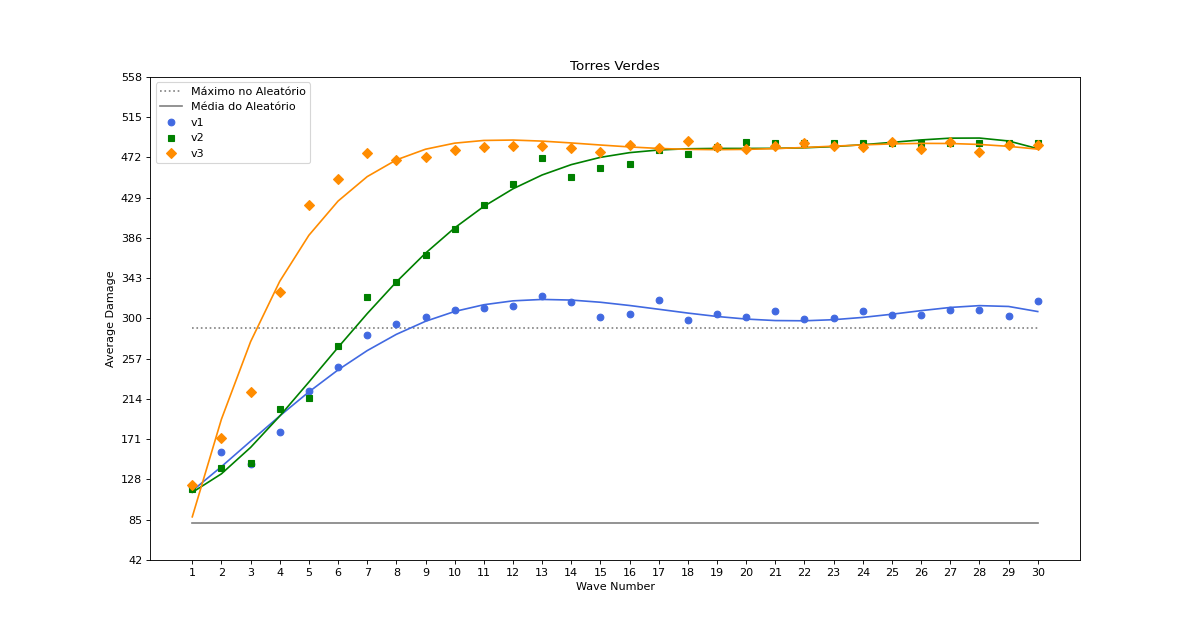
\includegraphics[width=1.1\textwidth]{td/Torres Verdes Fitness.png}
  \caption{Gráfico com as médias de dano para cada onda no teste com as Torres Verdes para as versões v1, v2 e v3.}
  \label{fig:fit-td-verde}
\end{figure}

\begin{figure}[H]
  \centering
  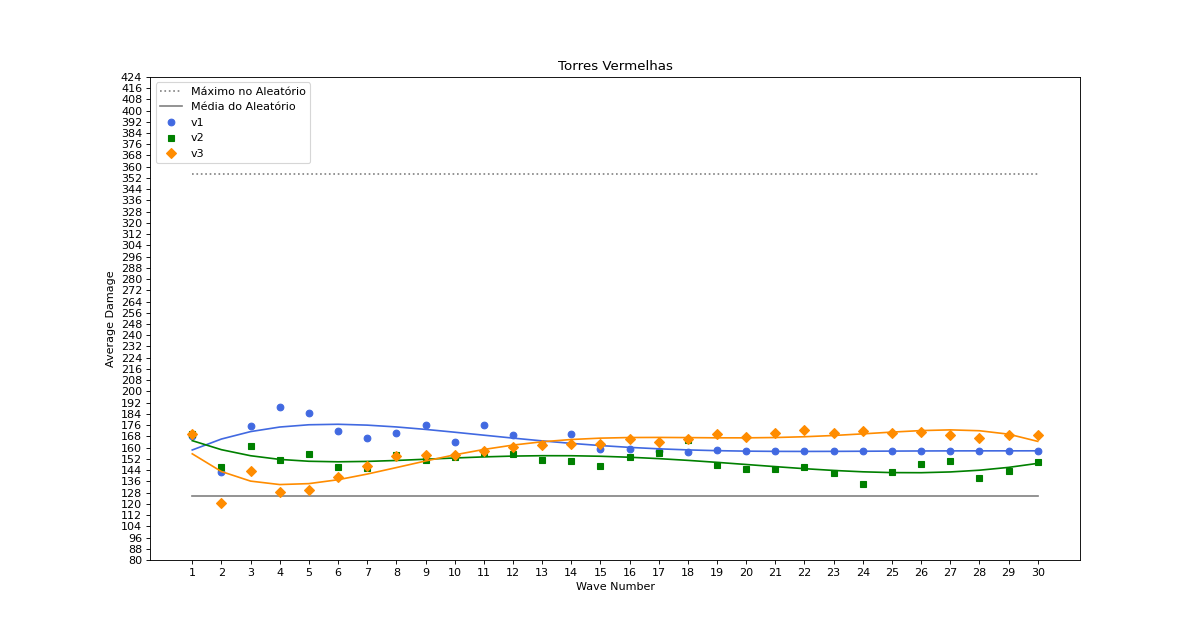
\includegraphics[width=1.1\textwidth]{td/Torres Vermelhas Fitness.png}
  \caption{Gráfico com as médias de dano para cada onda no teste com as Torres Vermelhas para as versões v1, v2 e v3.}
  \label{fig:fit-td-verm}
\end{figure}

\begin{figure}[H]
  \centering
  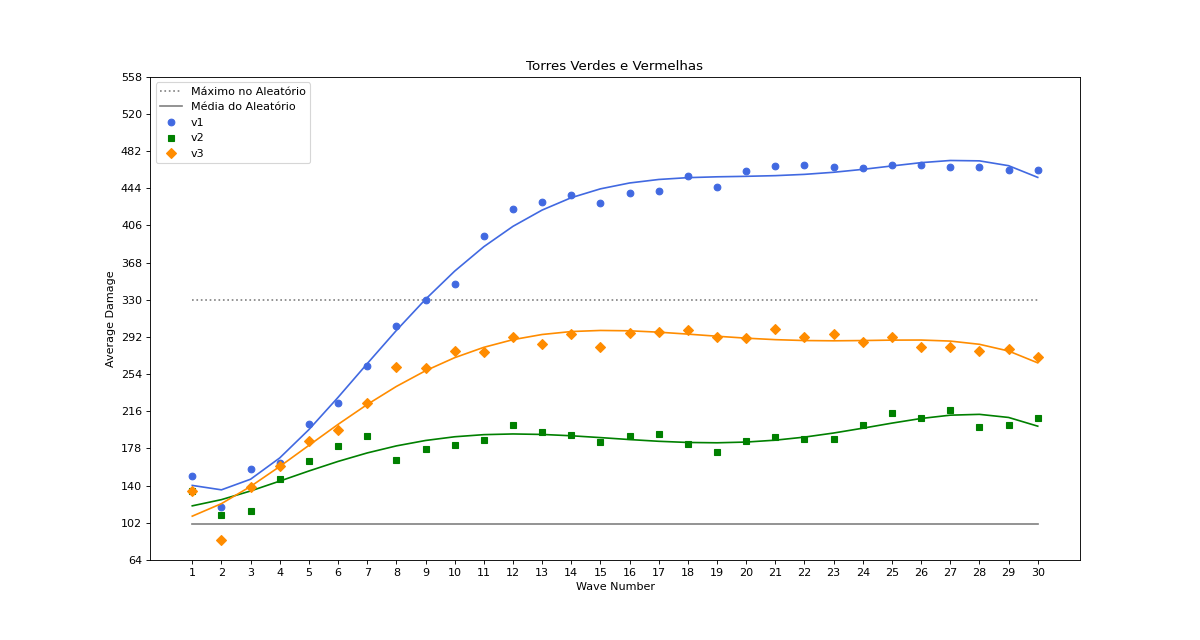
\includegraphics[width=1.1\textwidth]{td/Torres Verdes e Vermelhas Fitness.png}
  \caption{Gráfico com as médias de dano para cada onda no teste com as Torres Verdes + Vermelhas para as versões v1, v2 e v3.}
  \label{fig:fit-td-verd-verm}
\end{figure}

\begin{figure}[H]
  \centering
  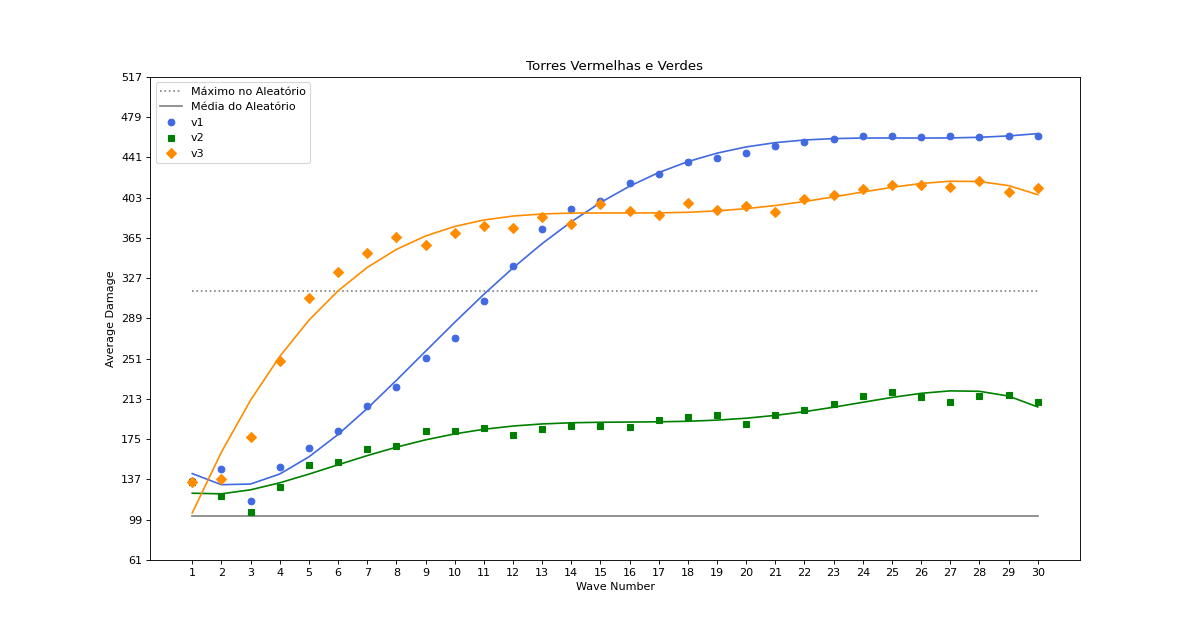
\includegraphics[width=1.1\textwidth]{td/Torres Vermelhas e Verdes Fitness.png}
  \caption{Gráfico com as médias de dano para cada onda no teste com as Torres Vermelhas + Verdes para as versões v1, v2 e v3.}
  \label{fig:fit-td-verm-verd}
\end{figure}

As Figuras \ref{fig:td-box-green}, \ref{fig:td-box-red}, \ref{td-box-gr} e \ref{td-box-rg} a seguir mostram o comportamento, em cada teste, do dano total de cada i-ésima onda, cada uma sendo representada num \textit{boxplot}.

\vfill
\pagebreak

\begin{figure}[H]
  \centering
  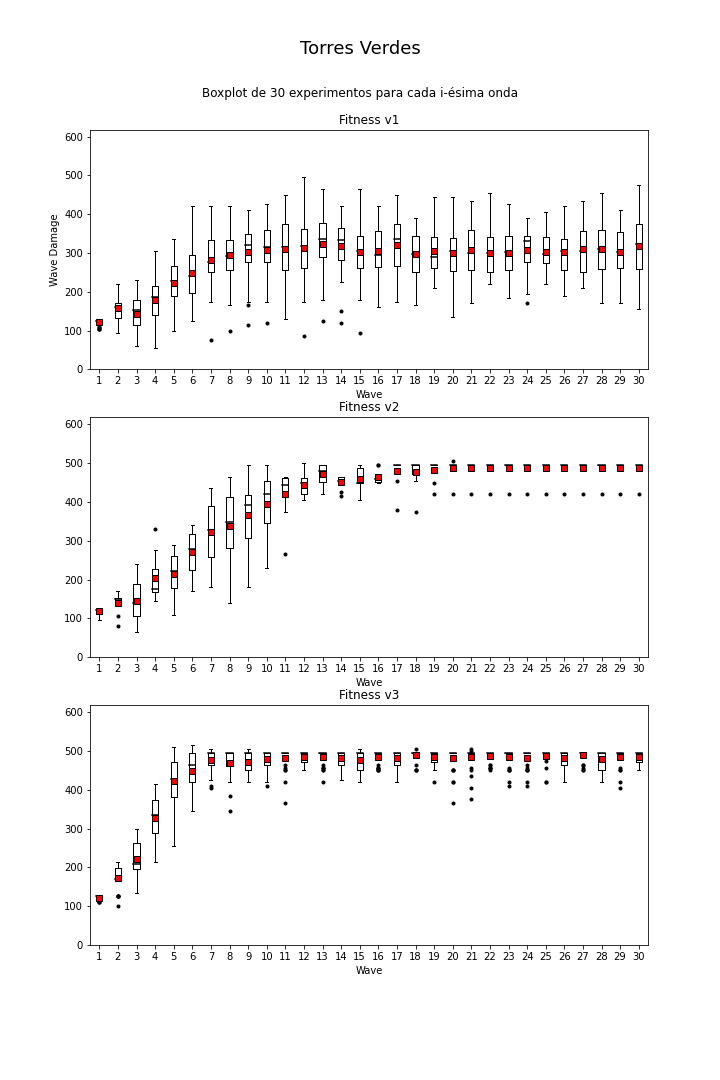
\includegraphics[width=1.1\textwidth]{figuras/td/boxplot Torres Verdes.png}
  \caption{Boxplot do dano das 30 ondas nos 30 experimentos, para as versões v1, v2 e v3.}
  \label{fig:td-box-green}
\end{figure}

\begin{figure}[H]
  \centering
  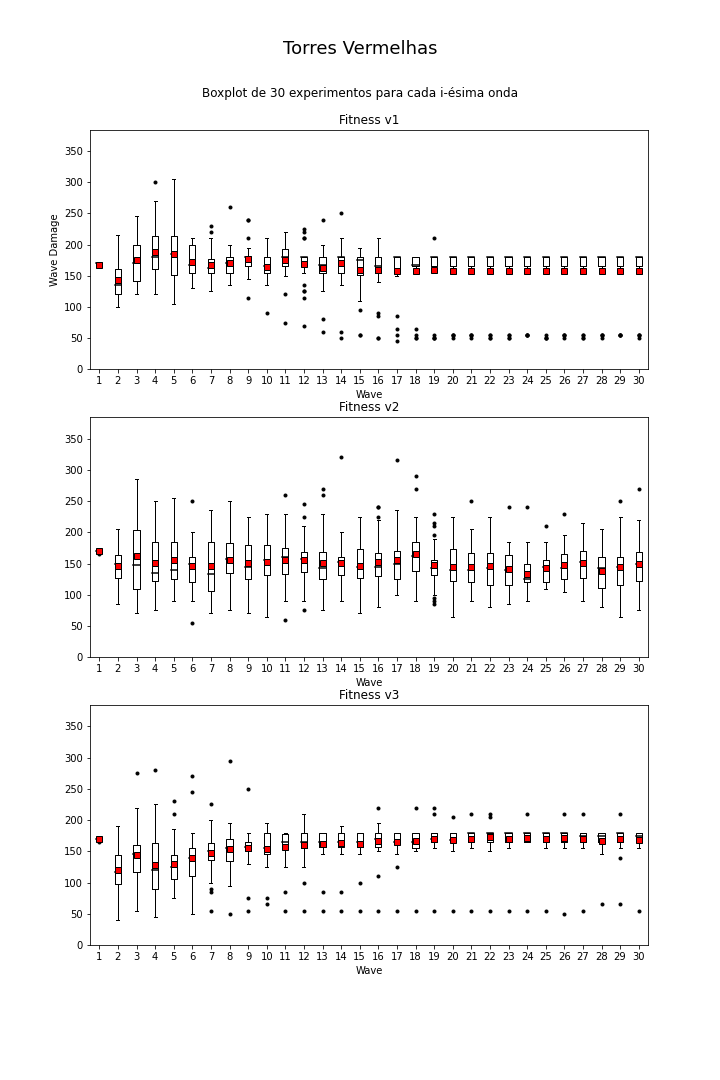
\includegraphics[width=1.1\textwidth]{figuras/td/boxplot Torres Vermelhas.png}
  \caption{Boxplot do dano das 30 ondas nos 30 experimentos, para as versões v1, v2 e v3.}
  \label{fig:td-box-red}
\end{figure}

\begin{figure}[H]
  \centering
  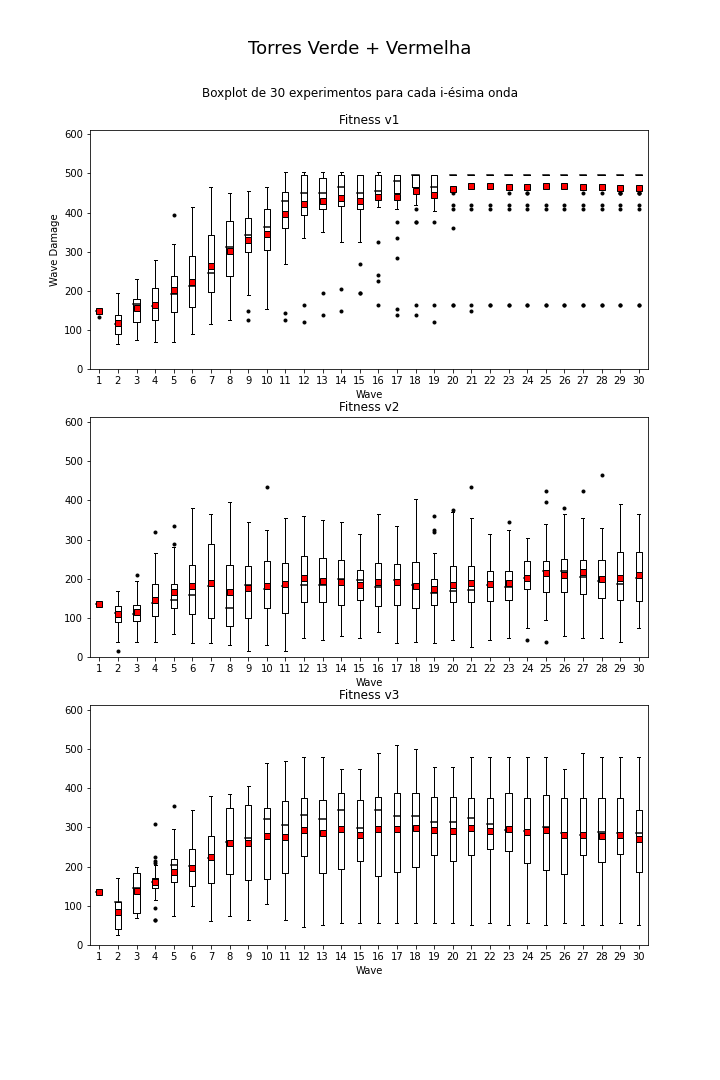
\includegraphics[width=1.1\textwidth]{figuras/td/boxplot Torres Verde + Vermelha.png}
  \caption{Boxplot do dano das 30 ondas nos 30 experimentos, para as versões v1, v2 e v3.}
  \label{td-box-gr}
\end{figure}

\begin{figure}[H]
  \centering
  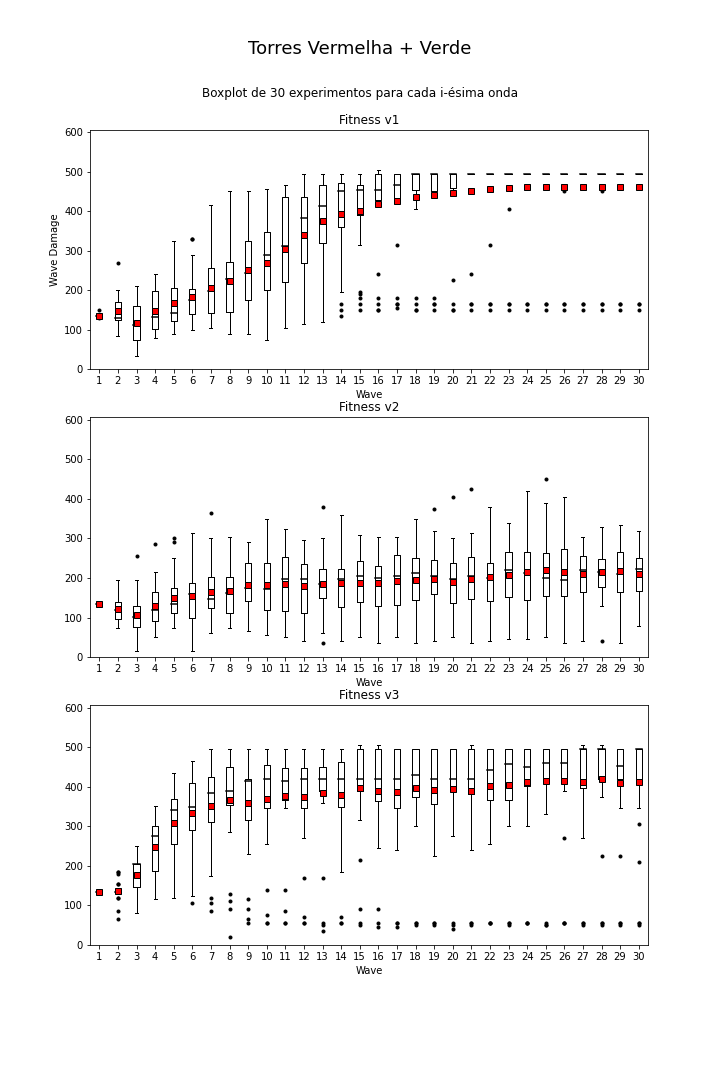
\includegraphics[width=1.1\textwidth]{figuras/td/boxplot Torres Vermelha + Verde.png}
  \caption{Boxplot do dano das 30 ondas nos 30 experimentos, para as versões v1, v2 e v3.}
  \label{td-box-rg}
\end{figure}

A Tabela \ref{tab:td-conver} mostra a onda aproximada onde o algoritmo parece ter convergido, e o dano médio após a estabilidade:

\begin{table}
\centering
\begin{tabular}{l|ll|ll|ll}
\multirow{2}{*}{Torres}                                     & \multicolumn{2}{l|}{v1} & \multicolumn{2}{l|}{v2} & \multicolumn{2}{l}{v3} \\
                                                            & Convergiu  & Dano Médio & Convergiu  & Dano Médio & Convergiu & Dano Médio \\ \hline
Verdes                                                      & 8          & 307.04     & 12         & 478.61     & 8         & 482.57     \\ \cline{1-7}
Vermelha                                                    & 15         & 157.78     & Não        & -          & 12        & 167.44     \\ \cline{1-7}
\begin{tabular}[c]{@{}l@{}}Verde +\\ Vermelha\end{tabular}  & 18         & 463.26     & Não        & -          & 11        & 288.18     \\ \cline{1-7}
\begin{tabular}[c]{@{}l@{}}Vermelha\\  + Verde\end{tabular} & 21         & 459.30     & Não        & -          & 12        & 399.16    
\end{tabular}
\caption{Tabela mostrando a onda onde ocorreu a convergência e o dano médio a partir desse ponto até o final.}
\label{tab:td-conver}
\end{table}

%% ------------------------------------------------------------------------- %%
\subsection{Tower Defense - Comparação}
\label{sec:td-fit-comp}

No \textit{Tower Defense} todas as versões do Algoritmos Genéticos se mostraram adequadas, superando a média da geração aleatória, entretanto no teste com Torres Vermelhas nenhuma superou o maior dano obtido em uma onda do teste \textit{Random}. Contra Torres Verdes existe uma solução ótima óbvia, tanques Verdes (\textit{EnemyGreen}), onde o inimigo com maior resistência (e portanto vida) é o mesmo com o maior dano, e as três versões testadas parecem chegar nesse resultado. 

Individualmente, as seguintes características foram apresentadas:

v1:
\begin{itemize}
  \item Convergência em todos os testes;
  \item Contra Torres Verdes apresenta a maior dispersão comparado com v2 e v3, mas o maior dano médio. Único caso onde a média e mediana ficaram próximas;
  \item Menor dispersão nos outros testes, após convergência;
  \item Exceto contra Torres Verdes, mostra dispersão inicial alta, quando converge concentra o dano no último quartil (Q4) e em \textit{outliers} próximos dos menores valores possíveis nas ondas repetidas, fornecidos na Tabela \ref{sec:uni-td}, mas com mediana acima da média;
  \item Não converge para um estado maximal contra Torres Vermelhas, mas consegue superar o maior dano aleatório (pois o melhor estado maximal detectado pela função \textit{fitness} é priorizar sobrevivência dos tanques ao invés do dano causado no Jogador);
  \item Maior dano, dentre as versões, contra Torres heterogêneas (Verde e Vermelha, Vermelha e Verde);
\end{itemize}

\pagebreak

v2:
\begin{itemize}
  \item Somente converge contra Torres Verdes - onde apresenta o segundo melhor resultado - concentrando resultados na mediana e em \textit{outliers} ligeiramente abaixo;
  \item Nos outros casos estabiliza de maneira oscilante, sem melhorar significativamente em relação a onda inicial, com poucos  \textit{outliers} mas muita dispersão (devido à taxa de mutação ser 100\% após a primeira onda);
  \item Consistente, com médias e medianas próximas.
\end{itemize}

v3:
\begin{itemize}
  \item Convergência em todos os testes, e mais rápida do que v1;
  \item Melhor resultado médio contra Torres Verdes - acima do maior dano aleatório - com dados concentrados no segundo e terceiro quartil, mediana acima da média e alguns \textit{outliers} ligeiramente abaixo;
  \item No teste contra Torres Vermelhas apresenta concentração de resultados entre a mediana no último quartil (Q4) e \textit{outliers} próximos das médias das piores ondas aleatórias;
  \item Apresenta a maior dispersão das versões do algoritmo contra Torres Verde + Vermelha, os quartis se estendendo desde o melhor resultado do v1 até os piores apresentados pelas ondas repetidas (Tabela \ref{sec:uni-td});
  \item Contra Torres Vermelha + Verde também supera o maior dano aleatório, com resultados concentrados entre a medianas no último quartil (Q4) e média, que foi afetada por \textit{outliers}.
\end{itemize}

Os resultados indicam que a versão v1 é bastante consistente, com baixa dispersão em 3 testes, mas corre risco de convergir em resultados longe do ótimo, possivelmente por progressivamente reduzir os genes aos piores candidatos e estabilizar no menos pior (taxa de mutação zera após a 20ª onda).

A última versão testada (v3) mostrou comportamento semelhante ao v1 mas com danos menores, exceto contra Torres Verdes. No restante não foi capaz de eliminar casos extremos onde estabilizou próximo do pior caso, apesar da pequena melhoria contra Torres Verde + Vermelha, provavelmente por reduzir os candidatos aptos por más escolhas, semelhante a v1.

\vfill
\pagebreak

%% ------------------------------------------------------------------------- %%
\subsection{Space Shooter - Resultados}
\label{sec:ss-fit-res}

Os gráficos seguintes (\ref{fig:fit-ss-ys}, \ref{fig:fit-ss-ym}, \ref{fig:fit-ss-rs} e \ref{fig:fit-ss-rm}) apresentam os resultados dos quatro casos de teste no jogo \textit{Space Shooter}, para as três opções citadas em \ref{sec:a-fitness-mutacao-usados}.

\begin{figure}[H]
  \centering
  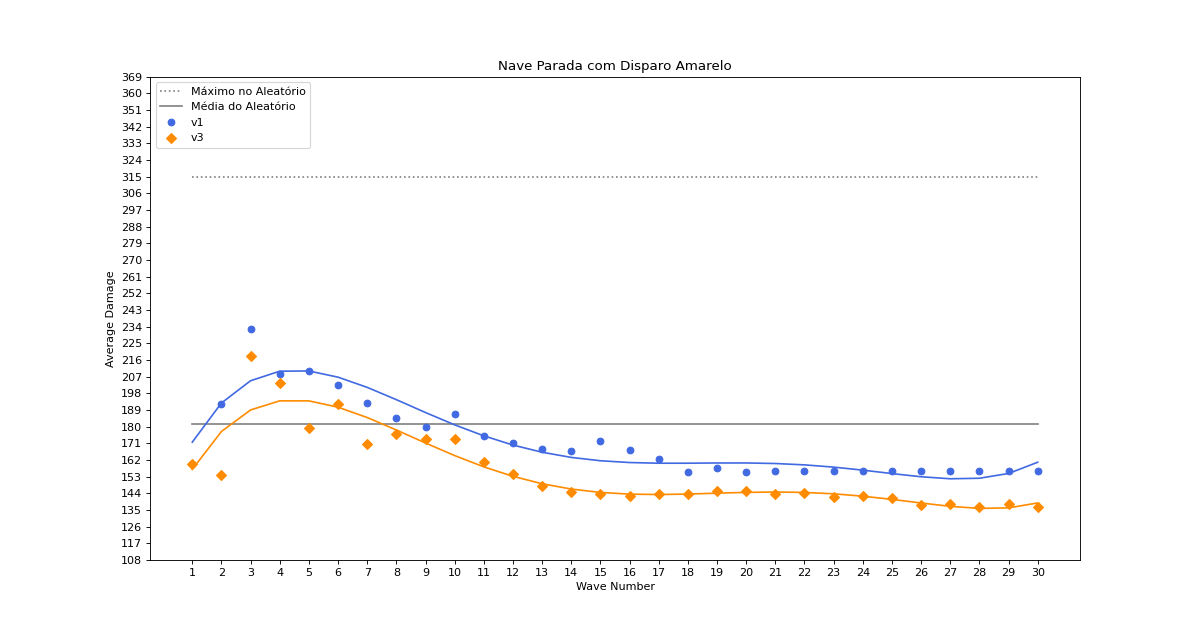
\includegraphics[width=1.1\textwidth]{ss/Nave Parada com Disparo Amarelo Fitness.png}
  \caption{Gráfico com as médias de dano para cada onda no teste com a Nave Parada, Disparo Amarelo para as versões v1 e v3.}
  \label{fig:fit-ss-ys}
\end{figure}

\begin{figure}[H]
  \centering
  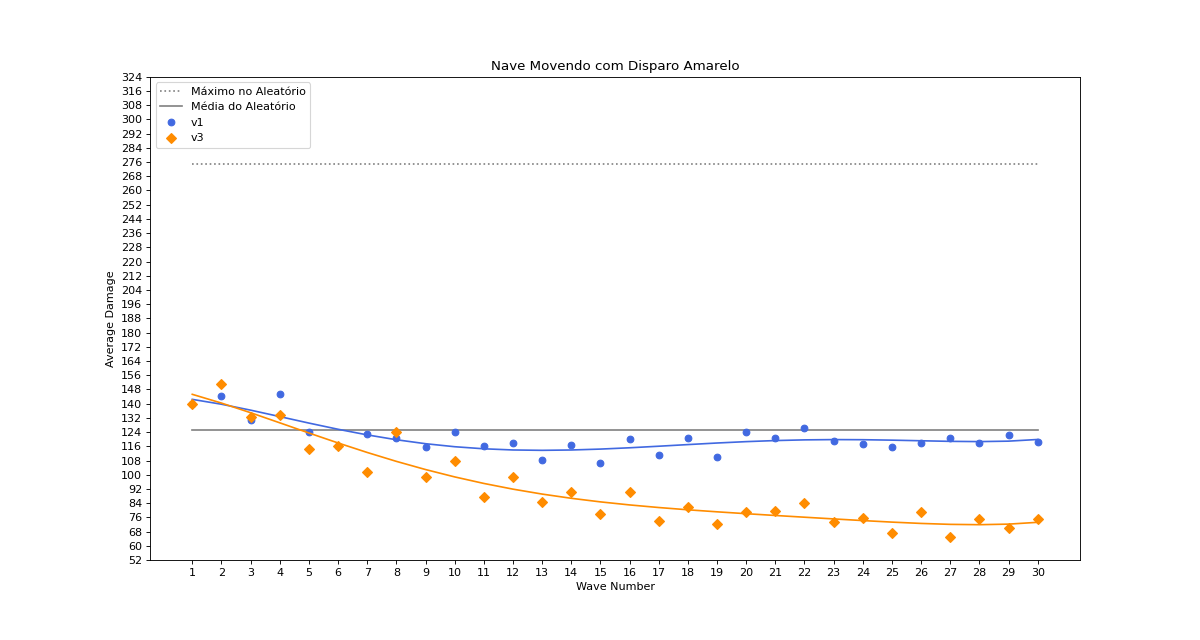
\includegraphics[width=1.1\textwidth]{ss/Nave Movendo com Disparo Amarelo Fitness.png}
  \caption{Gráfico com as médias de dano para cada onda no teste com a Nave Movendo, Disparo Amarelo para as versões v1 e v3.}
  \label{fig:fit-ss-ym}
\end{figure}

\begin{figure}[H]
  \centering
  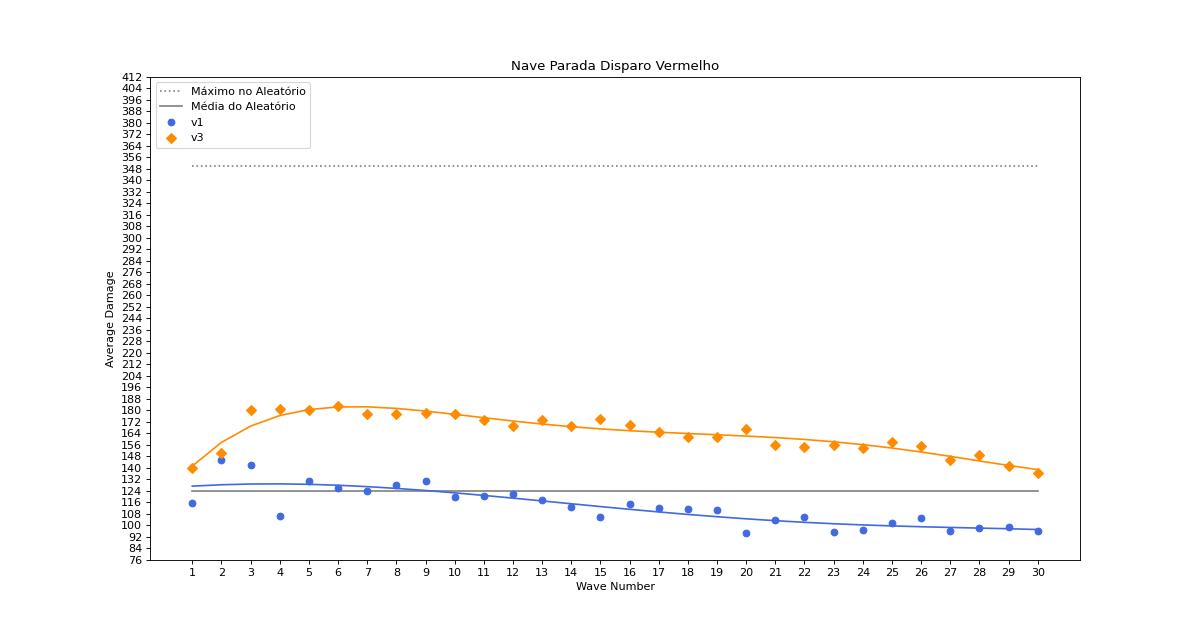
\includegraphics[width=1.1\textwidth]{ss/Nave Parada Disparo Vermelho Fitness.png}
  \caption{Gráfico com as médias de dano para cada onda no teste com a Nave Parada, Disparo Vermelho para as versões v1 e v3.}
  \label{fig:fit-ss-rs}
\end{figure}

\begin{figure}[H]
  \centering
  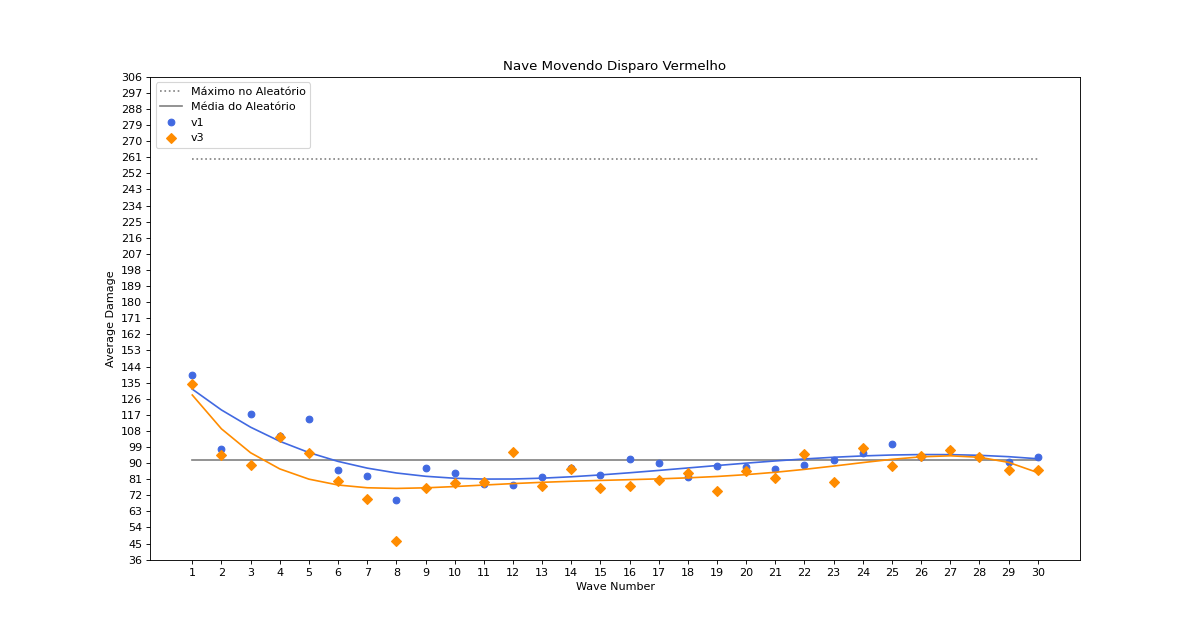
\includegraphics[width=1.1\textwidth]{ss/Nave Movendo Disparo Vermelho Fitness.png}
  \caption{Gráfico com as médias de dano para cada onda no teste com a Nave Movendo, Disparo Vermelho para as versões v1 e v3.}
  \label{fig:fit-ss-rm}
\end{figure}




Semelhante a Seção \ref{sec:td-fit-res}, as Figuras \ref{fig:ss-box-green}, \ref{fig:ss-box-red}, \ref{ss-box-gr} e \ref{ss-box-rg} a seguir mostram o comportamento, em cada teste, do dano total de cada i-ésima onda, cada uma sendo representada num \textit{boxplot}.

\begin{figure}
  \centering
  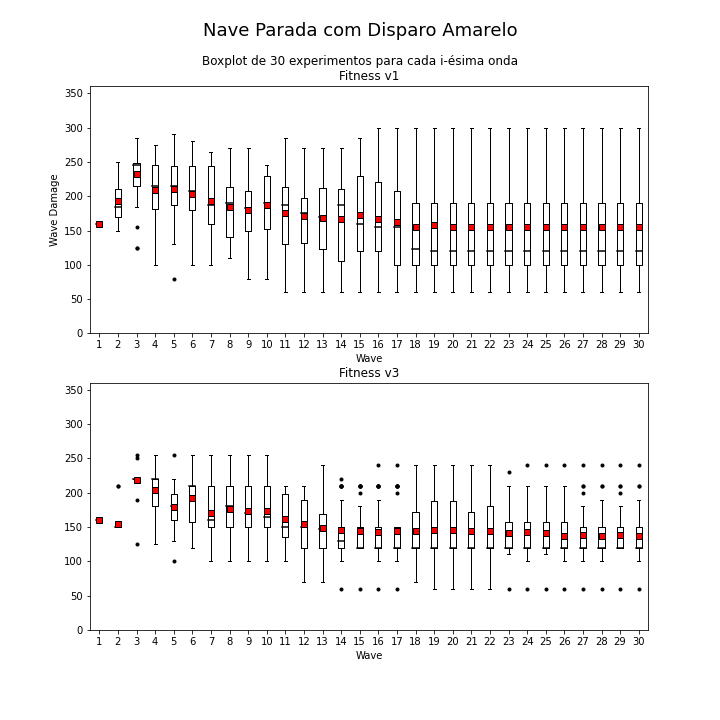
\includegraphics[width=1.1\textwidth]{figuras/ss/boxplot Nave Parada com Disparo Amarelo.png}
  \caption{Boxplot do dano das 30 ondas nos 30 experimentos, para as versões v1 e v3.}
  \label{fig:ss-box-green}
\end{figure}

\begin{figure}
  \centering
  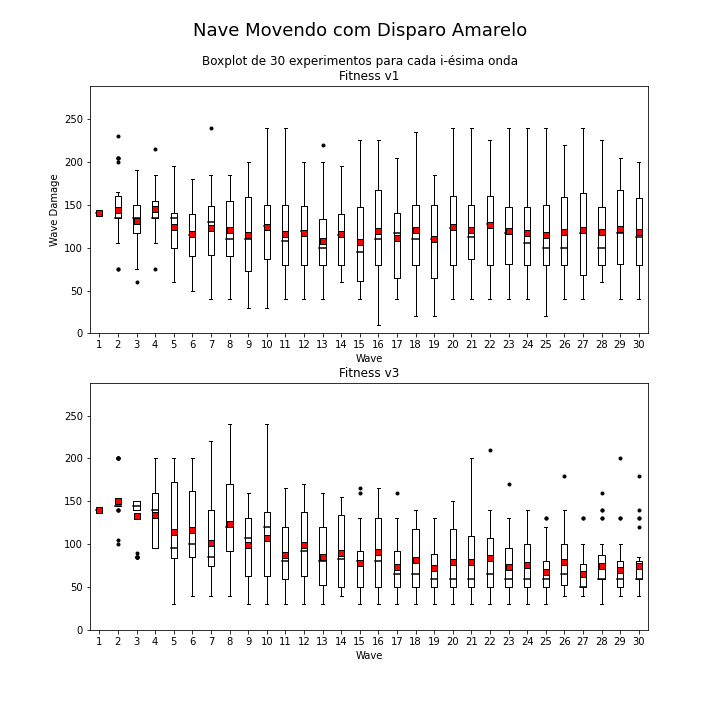
\includegraphics[width=1.1\textwidth]{figuras/ss/boxplot Nave Movendo com Disparo Amarelo.png}
  \caption{Boxplot do dano das 30 ondas nos 30 experimentos, para as versões v1 e v3.}
  \label{fig:ss-box-red}
\end{figure}

\begin{figure}
  \centering
  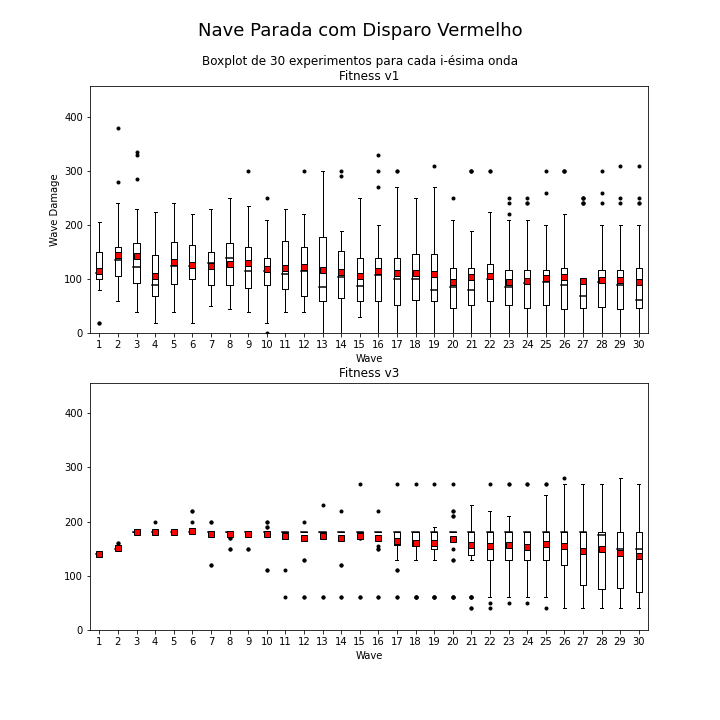
\includegraphics[width=1.1\textwidth]{figuras/ss/boxplot Nave Parada com Disparo Vermelho.png}
  \caption{Boxplot do dano das 30 ondas nos 30 experimentos, para as versões v1 e v3.}
  \label{ss-box-gr}
\end{figure}

\begin{figure}
  \centering
  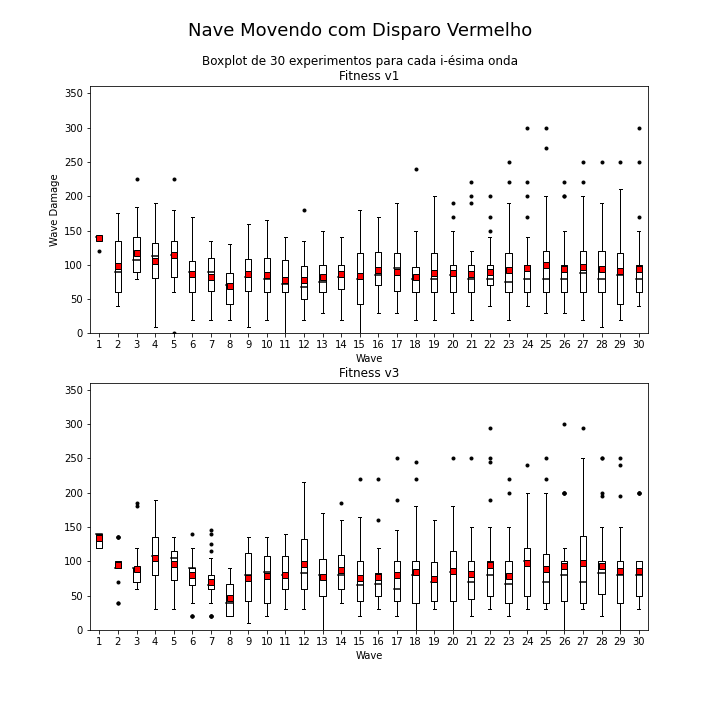
\includegraphics[width=1.1\textwidth]{figuras/ss/boxplot Nave Movendo com Disparo Vermelho.png}
  \caption{Boxplot do dano das 30 ondas nos 30 experimentos, para as versões v1 e v3.}
  \label{ss-box-rg}
\end{figure}

A Tabela \ref{tab:ss-conv} mostra a onda aproximada onde o algoritmo parece ter convergido, e o dano médio após a estabilidade:

\begin{table}
\centering
\begin{tabular}{l|ll|ll}
\multirow{2}{*}{Nave}                                              & \multicolumn{2}{l|}{v1} & \multicolumn{2}{l}{v3} \\
                                                                   & Convergiu  & Dano Médio & Convergiu & Dano Médio \\ \hline
\begin{tabular}[c]{@{}l@{}}Disparo Amarelo\\ Parada\end{tabular}   & 18         & 163.54     & 13        & 147.66     \\
\begin{tabular}[c]{@{}l@{}}Disparo Amarelo\\ Movendo\end{tabular}  & Não        & -          & Não       & -          \\
\begin{tabular}[c]{@{}l@{}}Disparo Vermelho\\ Parada\end{tabular}  & Não        & -          & Não       & -          \\
\begin{tabular}[c]{@{}l@{}}Disparo Vermelho\\ Movendo\end{tabular} & Não        & -          & Não       & -         
\end{tabular}
\caption{Tabela mostrando a onda onde ocorreu a convergência e o dano médio a partir desse ponto até o final.}
\label{tab:ss-conv}
\end{table}


%% ------------------------------------------------------------------------- %%
\subsection{Space Shooter - Comparação}
\label{sec:ss-fit-comp}

No \textit{Space Shooter} nenhuma versão do algoritmo genético se mostrou adequada pois as ondas convergiram em um ponto não maximal de dano causado, e, em somente um caso, conseguiram dano maior do que na geração aleatória, nunca atingindo o dano máximo de uma dessas ondas. Individualmente, as seguintes características foram apresentadas:

v1
\begin{itemize}
  \item Consegue obter o mesmo dano da onda aleatória em dois testes - Nave Parada com Disparo Amarelo e com Disparo Vermelho;
  \item Com Disparo Amarelo apresenta alta dispersão e poucos \textit{outliers}, com média acima da mediana;
  \item Em particular, com a Nave Parada o algoritmo converge a um resultado não maximal, mas consegue gerar ondas de dano total próximo do máximo teórico (360) \ref{sec:uni-ss} (possivelmente, por priorizar os inimigos que sobrevivem mais ao invés de os que causam mais dano, uma vez que a função \textit{fitness} não prioriza o dano que cada tipo de inimigo causa);
  \item Em geral estabiliza de maneira oscilante, com ondas melhores e piores de maneira sequencial, e médias acima da mediana;
  \item Estabiliza com oscilação e taxa de dano decrescente no teste contra a Nave Parada e Disparo Vermelho, no entanto com diversas ondas que foram totalmente eliminadas, e algumas com dano próximo do máximo (um caso interessante, pois existem alguns tipos de inimigos que sobrevivem melhor em conjunto com outros tipos, mas morrem quando sozinhos e que se reproduz na natureza também, como a co-extinção);
\end{itemize}

\pagebreak

v3
\begin{itemize}
  \item No geral apresenta dispersão menos uniforme do que v1, com maior presença de \textit{outliers};
  \item Com disparo amarelo mantém média bastante acima da mediana, mas não chega a produzir ondas próximas ao máximo como v1, apesar de reduzir ocorrências de inimigos fracos;
  \item Converge no teste com Nave Parada e Disparo Amarelo;
  \item Apresenta o único dano acima da onda aleatória entre todos os testes contra a Nave Parada e Disparo Vermelho, onde possui pouca variação até a onda 10, quando começam \textit{outliers}, e a partir da 20 aumenta drasticamente a dispersão;
  \item Estabiliza de maneira oscilante, com taxa decrescente de dano nos testes com Nave Parada e Disparo Amarelo e Nave Movendo com Disparo Vermelho;
  \item Praticamente empata com o gerador aleatório no teste com a Nave Movendo e Disparo Vermelho, mas de maneira oscilante e viés decrescente, apresentando \textit{outliers} próximos do dano máximo possível.
\end{itemize}

Ambos os \textit{fitness} apresentam comportamento semelhante, onde as ondas iniciais melhoram os resultados coletivos - o dano total - mas progressivamente perdem eficiência, possivelmente devido a tentativa do algoritmo buscar os resultados melhores individuais mas sem a capacidade de detectar que a ordem de aparecimento potencializa o dano, pois a nave só pode atirar no asteroide que apareceu primeiro em seu raio de visão. Logo, é possível que um inimigo lento seguido de outros velozes maximizem o dano de uma rodada, ao "distrair" o jogador, mas que numa avaliação individual essa sequência de inimigos perca para outra onde um inimigo mais forte atingiu o jogador.

O Disparo Vermelho, que possui maior potência, pode ter produzido resultados fracos pois ondas que são totalmente eliminadas não oferecem oportunidade a detecção de candidatos para novas gerações, deixando o algoritmo sem opções de escolha.





